\documentclass[11pt]{article}
\usepackage{fullpage}
\usepackage{graphicx}
\usepackage{amsmath}
\usepackage{times}
\usepackage{url}
\usepackage{latexsym}
\usepackage{amssymb}
\usepackage{amsthm}
\usepackage{tikz}
\usetikzlibrary{automata, positioning, arrows}

\begin{document}

\title{Assignment 1 \\ NLP 201:  Natural Language Processing I}

\author{}

\date{Out: October 13, 2020\\
      Due: October 27, 2020 11:59pm}
\maketitle

\textbf{All assignments are to be completed individually. You may discuss with the TAs and the instructor, but you may not receive help from anyone else.}

\paragraph{Instructions.} Create a \LaTeX-typeset write-up of your solutions and submit it to Canvas. Some free tools that might help: TexStudio (Windows), MacTex (Mac), TeX Live (cross-platform), and Overleaf (online). For the problems that require that you give FSAs, we encourage you to create them using drawing tools such as OmniGraffle (Mac) or yEd (online or cross-platform), but we will accept hand-drawn figures for full credit. Make sure initial and final states are clearly identified and explicitly list all symbols on each arc (i.e., no wildcards). We ask that you do not use any automated tools to \emph{solve} these problems as you will not have access to such tools for similar problems on the exams.


\section*{Problem 1 [15 points]}
For the following NFA containing $\varepsilon$-moves,

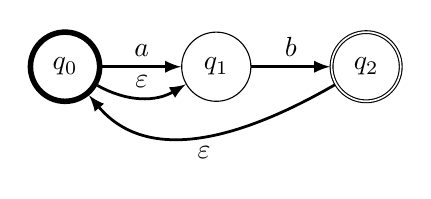
\begin{tikzpicture}

    \node(q0)[state,line width=2pt]{$q_0$};
    \node(q1)[state,right=of q0]{$q_1$};
    \node(q2)[state,accepting,right=of q1]{$q_2$};

    \draw (q0) edge[-latex, line width=1pt, bend right, above] node{$\varepsilon$} (q1)
          (q0) edge[-latex, line width=1pt,  above] node{$a$} (q1)
          (q1) edge[-latex, line width=1pt,  above] node{$b$} (q2)
          (q2) edge[-latex, line width=1pt, out=210,in=-50, below] node{$\varepsilon$} (q0)
          ;

\end{tikzpicture}



\noindent give an equivalent DFA.

\begin{tikzpicture}

  \node(q0q1)[state,line width=2pt,left=of q1]{$\{q_0,q_1\}$};
  \node(q1)[state,right=of q0q1]{$\{q_1\}$};
  \node(q2)[state,accepting,right=of q1]{$\{q_2\}$};
  \node(q0q1q2)[state,accepting,below=of q1]{$\{q_0,q_1,q_2\}$};
  \path[every loop/.append style=-{latex},
        every edge/.append style=-{latex}]

        (q0q1) edge[line width=1pt, below,right] node{$b$} (q0q1q2)
        (q0q1) edge[line width=1pt, above] node{$a$} (q1)

        (q1) edge[line width=1pt, bend left, above] node{$b$} (q2)

        (q2) edge[line width=1pt, bend left, below] node{$a$} (q1)
        (q2) edge[line width=1pt, loop right] node{$b$} (q2)

        (q0q1q2) edge[line width=1pt, loop right] node{$b$} (q0q1q2)
        (q0q1q2) edge[line width=1pt, left] node{$a$} (q1)
        ;

\end{tikzpicture}


\section*{Problem 2 [15 points]}

\noindent Give DFAs accepting the following languages.




\begin{enumerate}

\item {\bf [5 points]} The set of strings over the alphabet $\{a,b,c\}$ in which the substring $bc$ never occurs.

\begin{tikzpicture}

  \node(q0)[state,line width=2pt,left=of q1]{$q_0$} ;
  \node(dummy)[state, minimum size=8mm]{};
  \node(q1)[state,accepting,right=of q0]{$q_1$};
  \node(q2)[state,right=of q1]{$q_2$};

  \path[every loop/.append style=-{latex},
        every edge/.append style=-{latex}]

        (q0) edge[line width=1pt, loop left] node{$a,c$} (q1)
        (q0) edge[line width=1pt, bend left, above] node{$b$} (q1)

        (q1) edge[line width=1pt, bend left, below] node{$a$} (q0)
        (q1) edge[line width=1pt, loop above, above] node{$b$} (q1)
        (q1) edge[line width=1pt, above] node{$c$} (q2)

        (q2) edge[line width=1pt, loop right] node{$a,b,c$} (q2)
        ;

\end{tikzpicture}

\item {\bf [5 points]} The set of strings over the alphabet $\{1,7\}$ that end in $11711$.

\begin{tikzpicture}

  \node(q0)[state,line width=2pt,left=of q1]{$q_0$};
  \node(q1)[state,right=of q0]{$q_1$};
  \node(q2)[state,right=of q1]{$q_2$};
  \node(q3)[state,right=of q2]{$q_3$};
  \node(q4)[state,right=of q3]{$q_4$};
  \node(q5)[state,accepting,right=of q4]{$q_5$};

  \path[every loop/.append style=-{latex},
        every edge/.append style=-{latex}]
        %
        (q0) edge[line width=1pt, loop left] node{$7$} (q0)
        (q0) edge[line width=1pt, bend left, above] node{$1$} (q1)

        (q1) edge[line width=1pt, bend left, above] node{$1$} (q2)
        (q1) edge[line width=1pt, bend left, below] node{$7$} (q0)

        (q2) edge[line width=1pt, bend left, above] node{$7$} (q3)
        (q2) edge[line width=1pt, bend left, below] node{$1$} (q1)

        (q3) edge[line width=1pt, bend left, above] node{$1$} (q4)
        (q3) edge[line width=1pt, bend left, below, in=125,out=20] node{$7$} (q0)

        (q4) edge[line width=1pt, bend left, above] node{$1$} (q5)
        (q4) edge[line width=1pt, bend left, below, in=110,out=20] node{$7$} (q0)

        (q5) edge[line width=1pt, bend left, above,in=-130,out=-55] node{$7$} (q3)
        (q5) edge[line width=1pt, bend left, above,in=-130,out=-70] node{$1$} (q1)
        ;

\end{tikzpicture}

\item {\bf [5 points]} The set of strings over the alphabet $\{0, 1\}$ which are divisible by three
 when interpreted as a binary number (ignoring leading zeroes).

 For example $00000_b = 0$, which is divisible by 3, so $00000$ should be accepted.
$001001_b = 9$ and thus should be accepted also.
$101_b = 5$ is not divisible by 3 and thus should be rejected.

{\bf Note:} $\varepsilon$ should be interpreted as 0 and thus should be accepted.

\begin{tikzpicture}

  \node(q0)[state,line width=2pt,left=of q1]{$q_0$} ;
  \node(dummy)[state, minimum size=8mm]{};
  \node(q1)[state,right=of q0]{$q_1$};
  \node(q2)[state,right=of q1]{$q_2$};

  \path[every loop/.append style=-{latex},
        every edge/.append style=-{latex}]

        (q0) edge[line width=1pt, loop left] node{$0$} (q1)
        (q0) edge[line width=1pt, bend left, above] node{$1$} (q1)

        (q1) edge[line width=1pt, bend left, below] node{$1$} (q0)
        (q1) edge[line width=1pt, bend left, above] node{$0$} (q2)

        (q2) edge[line width=1pt, bend left, below] node{$0$} (q1)
        (q2) edge[line width=1pt, loop right] node{$1$} (q2)

        ;

\end{tikzpicture}

\end{enumerate}
\pagebreak
\section*{Problem 3 [10 points]}

Give a {\em non-deterministic} FSA (possibly with $\varepsilon$-moves) accepting
the following language.

\begin{enumerate}

\item The set of strings over $\{1,7\}$ ending in $11711$.
How does your NFA differ from the DFA you constructed in Problem~2.2?

\begin{tikzpicture}

  \node(q0)[state,line width=2pt,left=of q1]{$q_0$};
  \node(q1)[state,right=of q0]{$q_1$};
  \node(q2)[state,right=of q1]{$q_2$};
  \node(q3)[state,right=of q2]{$q_3$};
  \node(q4)[state,right=of q3]{$q_4$};
  \node(q5)[state,accepting,right=of q4]{$q_5$};

  \path[every loop/.append style=-{latex},
        every edge/.append style=-{latex}]
        %
        (q0) edge[line width=1pt, loop left] node{$1,7$} (q0)
        (q0) edge[line width=1pt, above] node{$1$} (q1)

        (q1) edge[line width=1pt, above] node{$1$} (q2)

        (q2) edge[line width=1pt,  above] node{$7$} (q3)

        (q3) edge[line width=1pt,  above] node{$1$} (q4)

        (q4) edge[line width=1pt, above] node{$1$} (q5)

        ;

\end{tikzpicture}

Because the ending of the string is the only part of any consequence, we ignore the first $n$ characters of the string until parsing $11711$ at the end. Since the FSA is non-deterministic, we only transition from $q_0$ to $q_1$ at this final substring. This stands in contrast to the deterministic FSA above, which must revert to previous states if the target substring is interrupted.


\end{enumerate}

\section*{Problem 4 [15 points]}

Give regular expressions for each of the following languages:

\begin{enumerate}

\item {\bf [7 points]} The set of strings over $\{a,b,c\}$ in which the
substring $bc$ never occurs.
\begin{verbatim}
((a|c)*|(a|c)*bb*a(a|c)*)
\end{verbatim}

\item {\bf [8 points]} The language described in Problem~2.3:
The set of strings over $\{0, 1\}$ which are divisible by three
 when interpreted as a binary number (ignoring leading zeroes).

For example $00000_b = 0$, which is divisible by 3, so $00000$ should be accepted.
$001001_b = 9$, and thus should be accepted also.
$101_b = 5$, is not divisible by 3, and thus should be rejected.

{\bf Note:} $\varepsilon$ should be interpreted as 0, and thus should be accepted.
\begin{verbatim}
0*(1(01*0)*1)*0*
\end{verbatim}
\end{enumerate}

\pagebreak

\section*{Problem 5 [20 points]}

We may define \textbf{generalized regular expressions} (GREs) as follows:
\begin{enumerate}
\item $\emptyset$ is a GRE denoting the empty language;
\item $\varepsilon$ is a GRE denoting the language $\{ \varepsilon \}$;
\item for each $\sigma \in \Sigma$, $\sigma$ is a GRE denoting the language $\{ \sigma \}$;
\item if $\alpha$ and $\beta$ are GREs, denoting the languages $A$ and $B$, respectively, then
\begin{itemize}
\item $(\alpha \mid \beta)$ is a GRE denoting $A \cup B$;
\item $(\alpha \beta)$ is a GRE denoting $A.B$;
\item $\alpha^*$ is a GRE denoting $A^*$;
\item \textbf{[new]} $(\alpha \wedge \beta)$ is a GRE denoting $A \cap B$; and
\item \textbf{[new]} $\neg \alpha$ is a GRE denoting $\overline{A}$.
\end{itemize}
\end{enumerate}
Prove that the languages denoted by GREs are regular.
\\
\\
\noindent \textbf{Note:} you may use refer to the definitions and proofs about  REs we provided in class and only deal with the two new clauses in the generalized definition.


\begin{proof}
  To prove $A \cap B$ is regular, we will first prove (without loss of generality) that $\overline A$ is regular.

  Consider the following FSA, which accepts the language $A$:\newline

  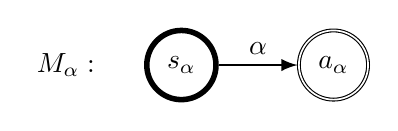
\begin{tikzpicture}
    \node(label1){$M_\alpha:$};
    \node(s_alpha)[state,line width=2pt,right=.5cm of label1]{$s_\alpha$};
    \node(a_alpha)[state,accepting,right=of s_alpha]{$a_\alpha$};

    \path[every loop/.append style=-{latex},
    every edge/.append style=-{latex}]

    (s_alpha) edge[line width=1pt, above] node{$\alpha$} (a_alpha)

    ;
  \end{tikzpicture}

  We then create a new FSA by swapping any accept states: \newline

  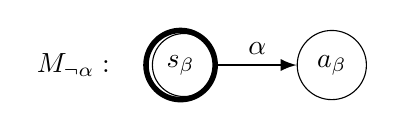
\begin{tikzpicture}
    \node(label3){$M_{\neg \alpha}:$};
    \node(s_negalpha)[state,line width=2pt,right=.3cm of label3]{$s_\beta$};
    \node(a_negalpha)[state,right=of s_negalpha]{$a_\beta$};
    \node(dummy)[state, minimum size=8mm, right=.41cm of label3]{};

    \path[every loop/.append style=-{latex},
    every edge/.append style=-{latex}]

    (s_negalpha) edge[line width=1pt, above] node{$\alpha$} (a_negalpha)
    ;
  \end{tikzpicture}

  This is a valid FSA, which accepts only the language of $\overline A$ (meaning $\overline A$ is regular).\newline

  Now we consider the language of $A \cap B$. Using De Morgan's Law we can show that $\overline {\overline A \cup \overline B} = A \cap B$.

  Because regular languages are known to be closed under union and complement, we can see that

  $A \cap B$ is also regular.


\end{proof}
\pagebreak
\section*{Problem 6 [25 points]}

For each of the following statements, answer whether the claim is {\bf true}
or {\bf false}, and give a {\em short} (one- to two-sentence) explanation if true or counterexample if false.

\begin{enumerate}

\item {\bf [5 points]} Let $L_1 \subset L_2$.  If $L_1$ is not regular, then $L_2$ must also be not regular.

{\bf False}. Consider the languages $L_1 = \{0^n1^n \mid n \in \mathbb N\}$ and $L_2 = \{0^*1^*\}$. Then $L_1 \subset L_2$, but $L_1$ is irregular, but $L_2$ is regular.

\item {\bf [5 points]} $L = L_1 \cap L_2$.  If $L_1$ and $L$ are regular languages, then $L_2$ must also be a regular language.


{\bf False}. Consider $L_1 = \{\varepsilon\}$ (regular) and $L_2 = \{0^n1^n\}$ (irregular). Then $L = L_1 \cap L_2 = \{\varepsilon\}$ (regular).


\item {\bf [5 points]} $L = L_1 \cup L_2$.  If $L_1$ and $L$ are regular languages, then $L_2$ must also be a regular language.


{\bf False}. Let $L_1 = \{0^n1^m\}$ (regular) and $L_2 = \{0^n1^n\}$ (irregular) for $n,m \in \mathbb N$ and $n<m$ (that is, $L_1 \subset L_2$). Then $L = L_1 \cup L_2 = \{0^n1^m\}$, which is still regular.


\item {\bf [5 points]} $L = \bigcap_{i=1}^{\infty} L_i$.  If all of the $L_i$
are regular languages, then $L$ is also a regular language.


{\bf False}. Let $L_i^p = \{0^n \mid n \leq i \text{ is prime}\}$ and $L_i^+ = \{0^n \mid n > i\}$. Define $L_i := L_i^p \cup L_i^+$. We see that $L_i^p$ is regular because it has finitely many prime-length words; $L_i^+$ is also clearly regular. As a result, $L_i$ is regular, being the union of two regular languages. However, we have $L = \bigcap_{i=1}^\infty L_i = \{0^p \mid p \text{ is prime}\}$, which is irregular by the pumping lemma.

\item  {\bf [5 points]}  Let $\alpha$, $\beta$ and $\gamma$ be regular expressions. If $L(\beta \mid \alpha \gamma) \subseteq L(\gamma)$, then $L(\alpha^* \beta) \subseteq L(\gamma)$.


{\bf True/False}.


\end{enumerate}

\end{document}
